\newpage
\section{Detektion von Snooker-Kugeln}\label{kap:detektion}
Aufgrund eines Bildes des Billardtisches soll der Spielstand mit der Position aller Kugeln bestimmt werden.
Der in dieser Arbeit verwendete Detektionsalgorithmus stammte von der vorherigen Projektarbeit\cite{project2:snooker_detection}
und funktioniert für Snooker-Kugeln.
In der Vorarbeit wurde die Detektion nur per Knopfdruck durchgeführt.
Mit dieser Arbeit wurde darauf aufbauend eine Live-Detektion implementiert, welche kontinuierlich Bilder vom Tisch macht,
den Spielstand detektiert und diesen dem Benutzer über den Projektor anzeigt.
Dadurch entsteht ein Feedback-Loop aufgrund der dargestellten Augmentationen im zu verarbeitenden Bild.
Ein Eingabebild für die Detektion ist in Abbildung \ref{fig:detection_feedback_loop} dargestellt und zeigt diesen Feedback-Loop.

\begin{figure}[h!]
    \begin{center}
        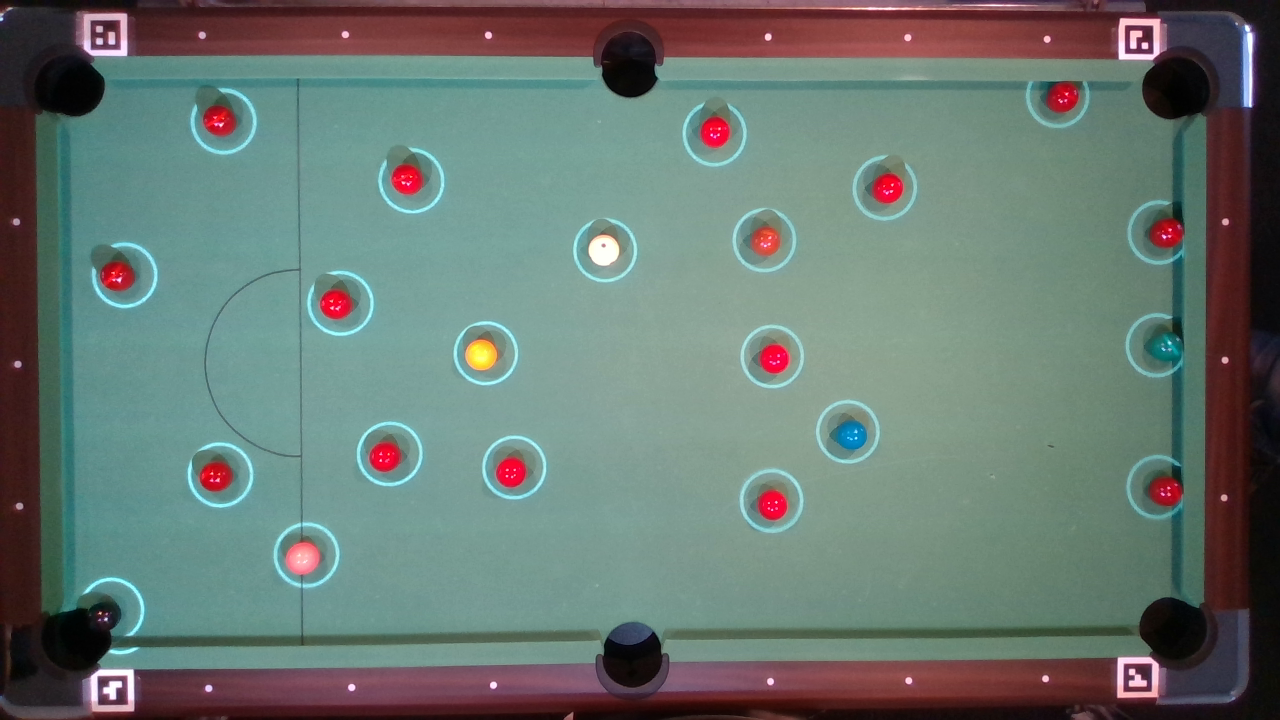
\includegraphics[width=0.8\linewidth]{../common/03_billiard_ai/resources/detection_feedback_loop.png}
    \end{center}
    \caption{Feedback-Loop in der Detektion}
    \label{fig:detection_feedback_loop}
\end{figure}

Die dargestellten Augmentationen können zu fälschlich detektierten Kugeln führen.
Um diesem Problem entgegenzuwirken, wurden die Parameter der Detektion höchstmöglich angepasst, um die Augmentationen
der fälschlich detektierten Kugeln so gering wie möglich zu halten.
Eine vollständige Eliminierung fälschlich detektierter Kugeln ist nicht möglich.

Des Weiteren wurde die Performance der Detektion erhöht, um die Live-Detektion aufzuwerten.
In der bisherigen Detektion wurden drei separate Circle Hough transform\cite{wiki:circle_hough} angewendet, eine für
jede der drei Gruppen von Kugeln, in die das Bild mittels Segmentation aufgeteilt wurde\cite{project2:snooker_detection}.
Zwei dieser drei konnten ohne einen bemerkbaren Verlust in der Qualität der Detektion zusammengefasst werden.
